\documentclass[12pt]{amsart}

%\usepackage{pdfsync}
\usepackage{latexsym,enumitem}
\usepackage{amssymb}
\usepackage[cp850]{inputenc}
\usepackage{epsfig}
\usepackage{psfrag}
\usepackage{amsthm}
\usepackage{amscd}
\usepackage{amsmath}
\usepackage{amsfonts}
\usepackage{graphics,caption}
\usepackage[all]{xy}
\usepackage{etoolbox}
\usepackage{xcolor}
\patchcmd{\quote}{\rightmargin}{\leftmargin 2em \rightmargin}{}{}
\captionsetup{width=4.7in}

\newtheorem{sat}{Theorem}[section]		\newtheorem{lem}[sat]{Lemma}
\newtheorem{kor}[sat]{Corollary}			\newtheorem{prop}[sat]{Proposition}
\newtheorem{bei}{Example}				\newtheorem{defi}[sat]{Definition}
\newtheorem{rmk}[sat]{Remark}
\newtheorem*{defi*}{Definition}			\newtheorem*{bei*}{Example}
\newtheorem*{sat*}{Theorem}				\newtheorem*{kor*}{Corollary}
\newtheorem*{rmk*}{Remark}				\newtheorem{quest}{Question}	
\newtheorem{claim}[sat]{Claim}	
\newtheorem{fact}[sat]{Fact}	

% number equations by section:
\renewcommand{\theequation}{\thesection.\arabic{equation}}
\let\ssection=\section
\renewcommand{\section}{\setcounter{equation}{0}\ssection}

\newtheorem*{namedtheorem}{\theoremname}
\newcommand{\theoremname}{testing}
\newenvironment{named}[1]{\renewcommand{\theoremname}{#1}\begin{namedtheorem}}{\end{namedtheorem}}

\theoremstyle{remark}
\newtheorem*{bem}{Remark}

%\setlength{\parindent}{0em}

%\newcommand{\defin}{\ensuremath{\overset{ \text{\tiny def} }{=} } }

\newcommand{\BC}{\mathbb C}			\newcommand{\BH}{\mathbb H}
\newcommand{\BR}{\mathbb R}			\newcommand{\BD}{\mathbb D}
\newcommand{\BN}{\mathbb N}			\newcommand{\BQ}{\mathbb Q}
\newcommand{\BS}{\mathbb S}			\newcommand{\BZ}{\mathbb Z}
\newcommand{\BF}{\mathbb F}			\newcommand{\BT}{\mathbb T}
\newcommand{\BU}{\mathbb U}
%\newcommand{\RP}{\mathrm P}

\newcommand{\CA}{\mathcal A}		\newcommand{\CB}{\mathcal B}
\newcommand{\CC}{\mathcal C}		\newcommand{\calD}{\mathcal D}
\newcommand{\CE}{\mathcal E}		\newcommand{\CF}{\mathcal F}
\newcommand{\CG}{\mathcal G}		\newcommand{\CH}{\mathcal H}
\newcommand{\CI}{\mathcal I}		\newcommand{\CJ}{\mathcal J}
\newcommand{\CK}{\mathcal K}		\newcommand{\CL}{\mathcal L}
\newcommand{\CM}{\mathcal M}		\newcommand{\CN}{\mathcal N}
\newcommand{\CO}{\mathcal O}		\newcommand{\CP}{\mathcal P}
\newcommand{\CQ}{\mathcal Q}		\newcommand{\CR}{\mathcal R}
\newcommand{\CS}{\mathcal S}		\newcommand{\CT}{\mathcal T}
\newcommand{\CU}{\mathcal U}		\newcommand{\CV}{\mathcal V}
\newcommand{\CW}{\mathcal W}		\newcommand{\CX}{\mathcal X}
\newcommand{\CY}{\mathcal Y}		\newcommand{\CZ}{\mathcal Z}

\newcommand{\actson}{\curvearrowright}
\newcommand{\D}{\partial}
\newcommand{\DD}{\nabla}
\newcommand{\into}{\hookrightarrow}


\DeclareMathOperator{\Out}{Out}		%	Aeussere Automorphismen einer Gruppe
\DeclareMathOperator{\Diff}{Diff}	%	Diffeomorphimen einer Mf
\DeclareMathOperator{\SL}{SL}		%	Spezielle lineare Gruppe
\DeclareMathOperator{\PSL}{PSL}		%	Spezielle lineare Gruppe
\DeclareMathOperator{\GL}{GL}		%	Allgemeine lineare Gruppe
\DeclareMathOperator{\Id}{Id}		%	Identit\"at
\DeclareMathOperator{\Isom}{Isom}	%	Isometrien einer Mf
\DeclareMathOperator{\Hom}{Hom}		%	Homomorphismen
\DeclareMathOperator{\vol}{vol}		%	Volumen
\DeclareMathOperator{\area}{area}
\DeclareMathOperator{\tr}{Tr}
\DeclareMathOperator{\SU}{SU}
\DeclareMathOperator{\Map}{Map}
\DeclareMathOperator{\inj}{inj}
\DeclareMathOperator{\diam}{diam}
\DeclareMathOperator{\rank}{rank}
\DeclareMathOperator{\Axis}{Axis}
\DeclareMathOperator{\maxrad}{maxrad}
\DeclareMathOperator{\height}{height}
\DeclareMathOperator{\rel}{rel}
\DeclareMathOperator{\arccosh}{arccosh}
\DeclareMathOperator{\Ker}{Ker}
\DeclareMathOperator{\diver}{div}
\DeclareMathOperator{\width}{width}
\DeclareMathOperator{\saturated}{Sat}
\DeclareMathOperator{\length}{length}

% \renewcommand\qedsymbol{\texttt{:-)}}



\begin{document}



\begin{sat}
	Let \(M\) be an irreducible compact manifold. Let \(F, F'\) be two incompressible compact, closed boundary components of \(M\). Suppose: if \(k\) is any closed curves in \(F\), then some non-null multiple of \(k\) is homotopic to a curve in \(F'\). Then \(M\) is homeomorphic to \(F\times I\).
\end{sat}

This is a weakened lemma from Waldhausen. In the original one, we did not assume compactness for \(M\) and \(F'\). However, in order to use the annulus theorem by Cannon-Feustel, we need \(M\) to be compact. Maybe it is not needed but I have not checked their proof yet.


\begin{proof}[Warm-up]
	 Suppose I am a student in intro to abstract math. I'm going to use the signature proof strategy: implicitly assume \(M = F \times I\), show that it satisfy the assumptions given, and then prove \(M \cong F \times I\). It is like we are doing a surgery on a lab rat to figure out what can work, and then try to apply to the more complicated case and try to resolve what don't work.
	 \begin{figure}[h!]
		\centering
		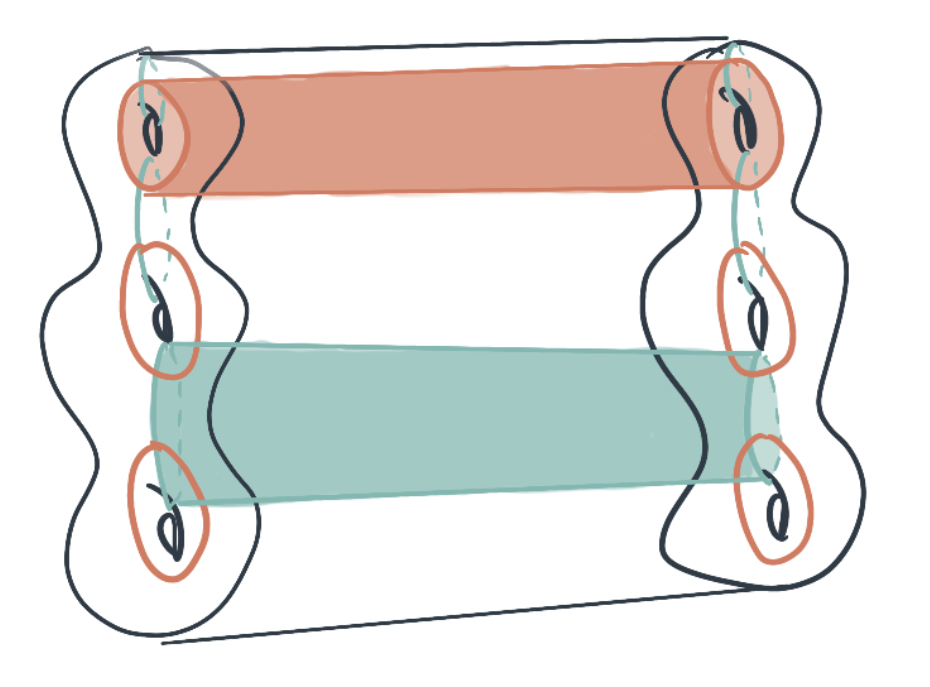
\includegraphics[width = 0.5\textwidth]{IMG1.png}
	 	\caption{(boring) cylinders in \(M = F\times I\).}
	 	\label{fig:cylinders}
	 \end{figure}

	 Suppose \(F\) has genus \(g\), then we can construct a system of essential simple closed curves \(k_1, \ldots, k_{2g}\) such that \(k_i\) and \(k_j\) intersect once traversely if \(i = j \pm 1\), and they are disjoint otherwise. If you have trouble finding such system, email me at \texttt{mujie.wang@bc.edu} for more assistance. For each \(k_j\), there is an annulus \(G_j = k_j \times I\) embedded in \(M\). See Figure \ref{fig:cylinders}. A pair of annuli \(G_i\) and \(G_j\) intersect if and only if \(k_i\) and \(k_j\) intersect, and the intersection \(G_i \cap G_j\) is exactly \((k_i \cap k_j)\times I\). 

	 Here comes the fun part! We want to show that if we cut out a regular neighborhood of two boundary components \(F_0, F_1 \cong F\) and all the annuli, what's left is a ball. First, consider 
	 \(\partial U(F_0 \cup \bigcup G_i) \cap \mathring{M}\), the boundary of regular neighborhood of \(F_0\) and the system of annuli in the interior of \(M\). It is homeomorphic to a bottle cap, which is homeomorphic to a disc. The top of the bottle cap comes from \(F_0 \backslash U(\bigcap k_j) \cong D^2\), which can be viewed as cutting \(F_0\) along this system of \(2g\) curves (with very blunt scissors) to get a disk. 
	 See Figure \ref{fig:disc}
	 The side of the bottle cap comes from \(\partial D^2 \times I\), which is homeomorphic to an annulus. Similarly, \(\partial U(F_1 \cup \bigcup G_i) \cap \mathring{M}\) is also homeomorphic to a disc. We will glue these two discs along \(\partial U(\bigcup G_i) \cap \mathring{M}\), which is{} homeomorphic to an annulus that can homotopy retract to both boundaries of the discs, since it is the part of both bottle caps minus the lids. Thus we conclude that \(\partial U(F_0 \cup F_1 \cup \bigcup G_i) \cap \mathring{M}\) is homeomorphic to \(S^2\), two disks glued at their boundaries . See Figure \ref{fig:bottlecap}. Since \(M = F\times I\) is irreducible, the complement of this regular neighborhood is the ball bounded by \(S^2\). 

	 \begin{figure}
	 	\centering
	 	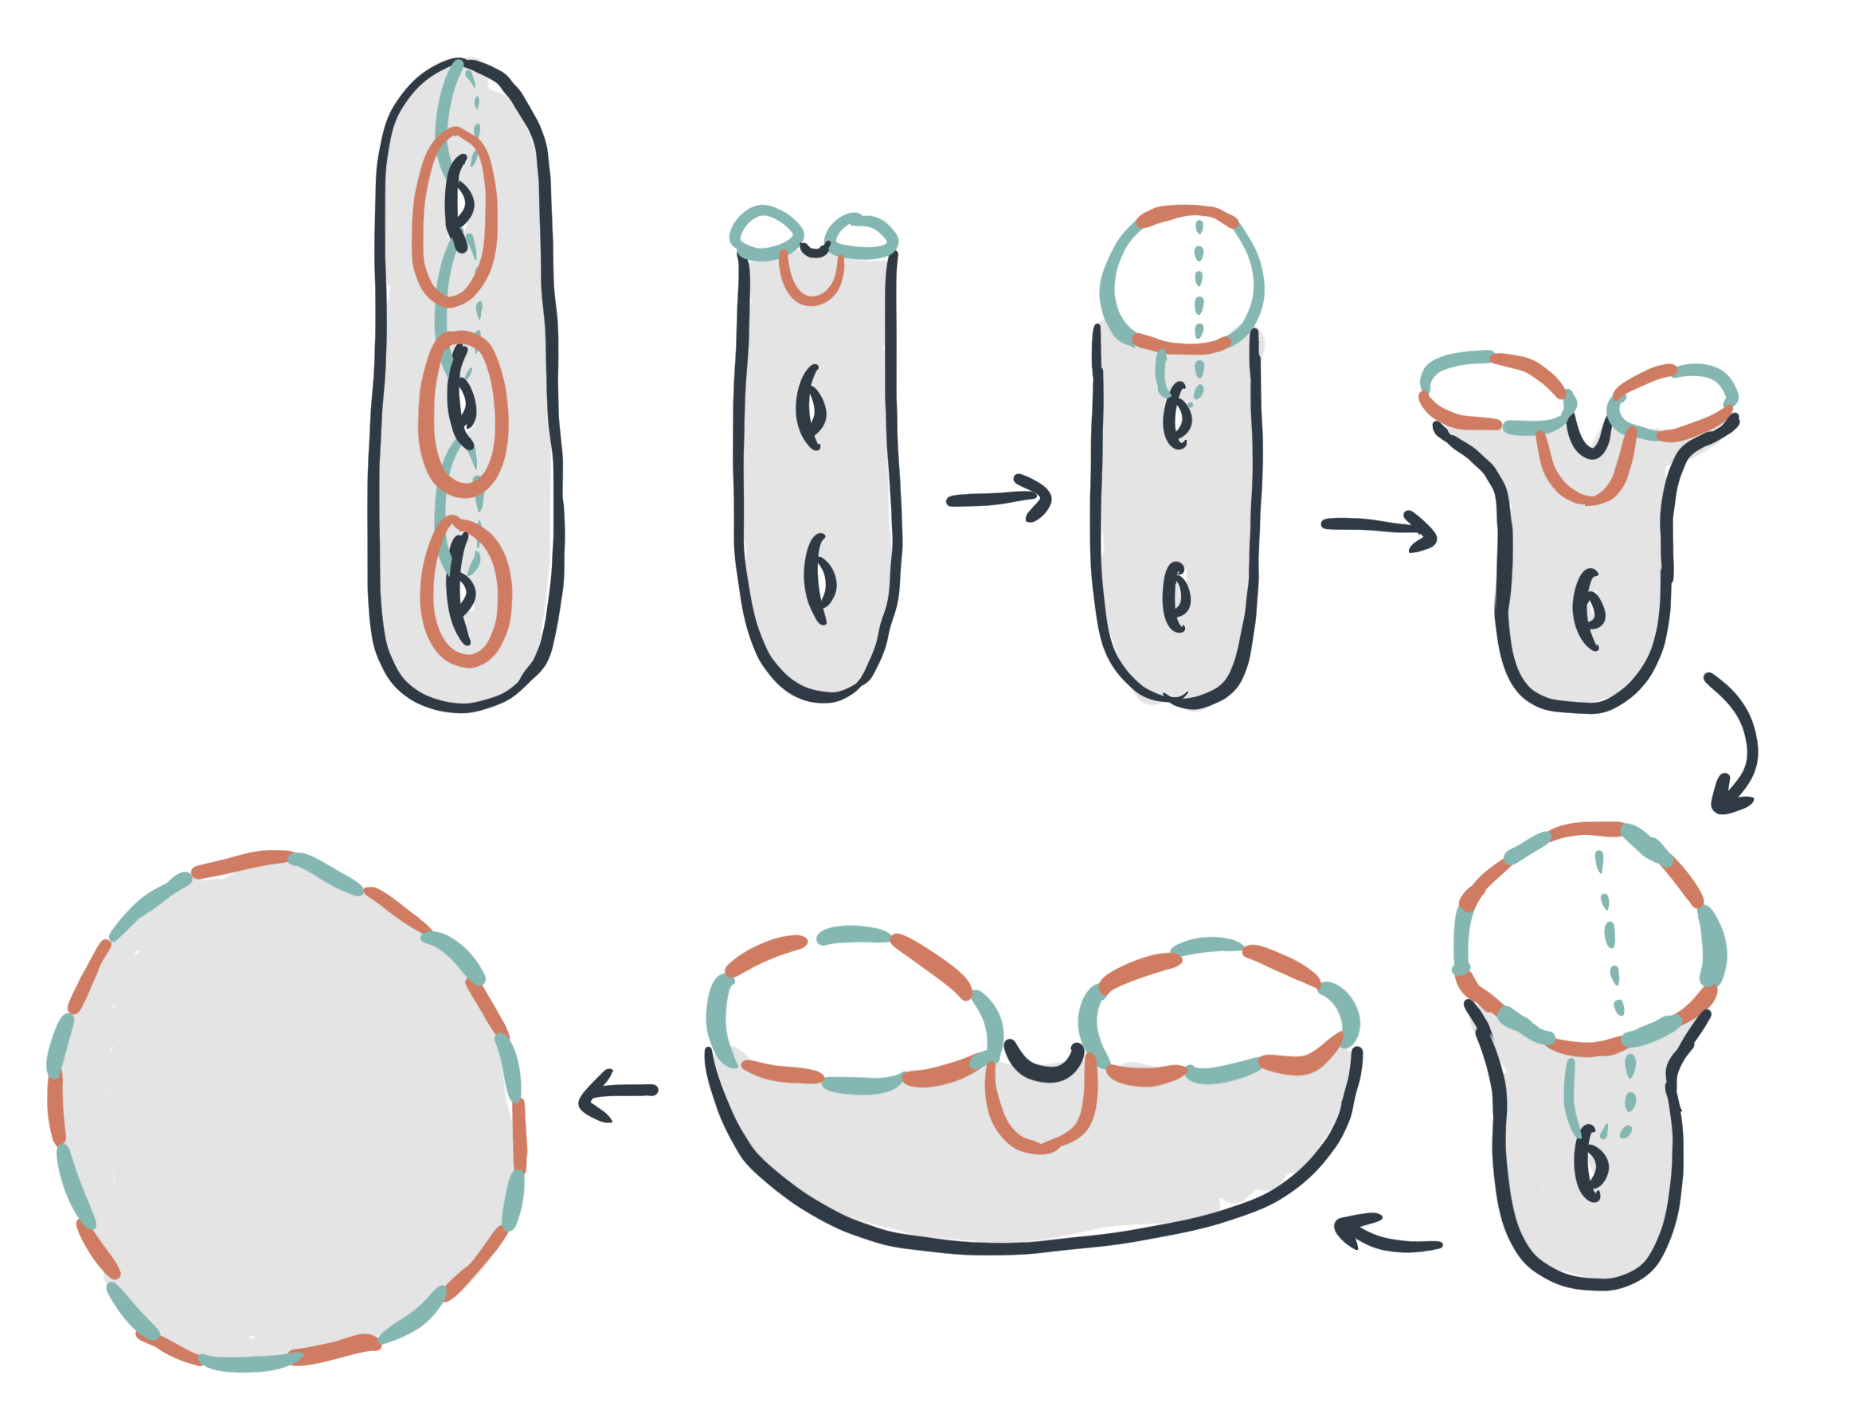
\includegraphics[width = 0.75\textwidth]{IMG3.png}
	 	\caption{cutting \(S_3\) along the system of curves.}
	 	\label{fig:disc}
	 \end{figure}

	 \begin{figure}
	 	\centering
	 	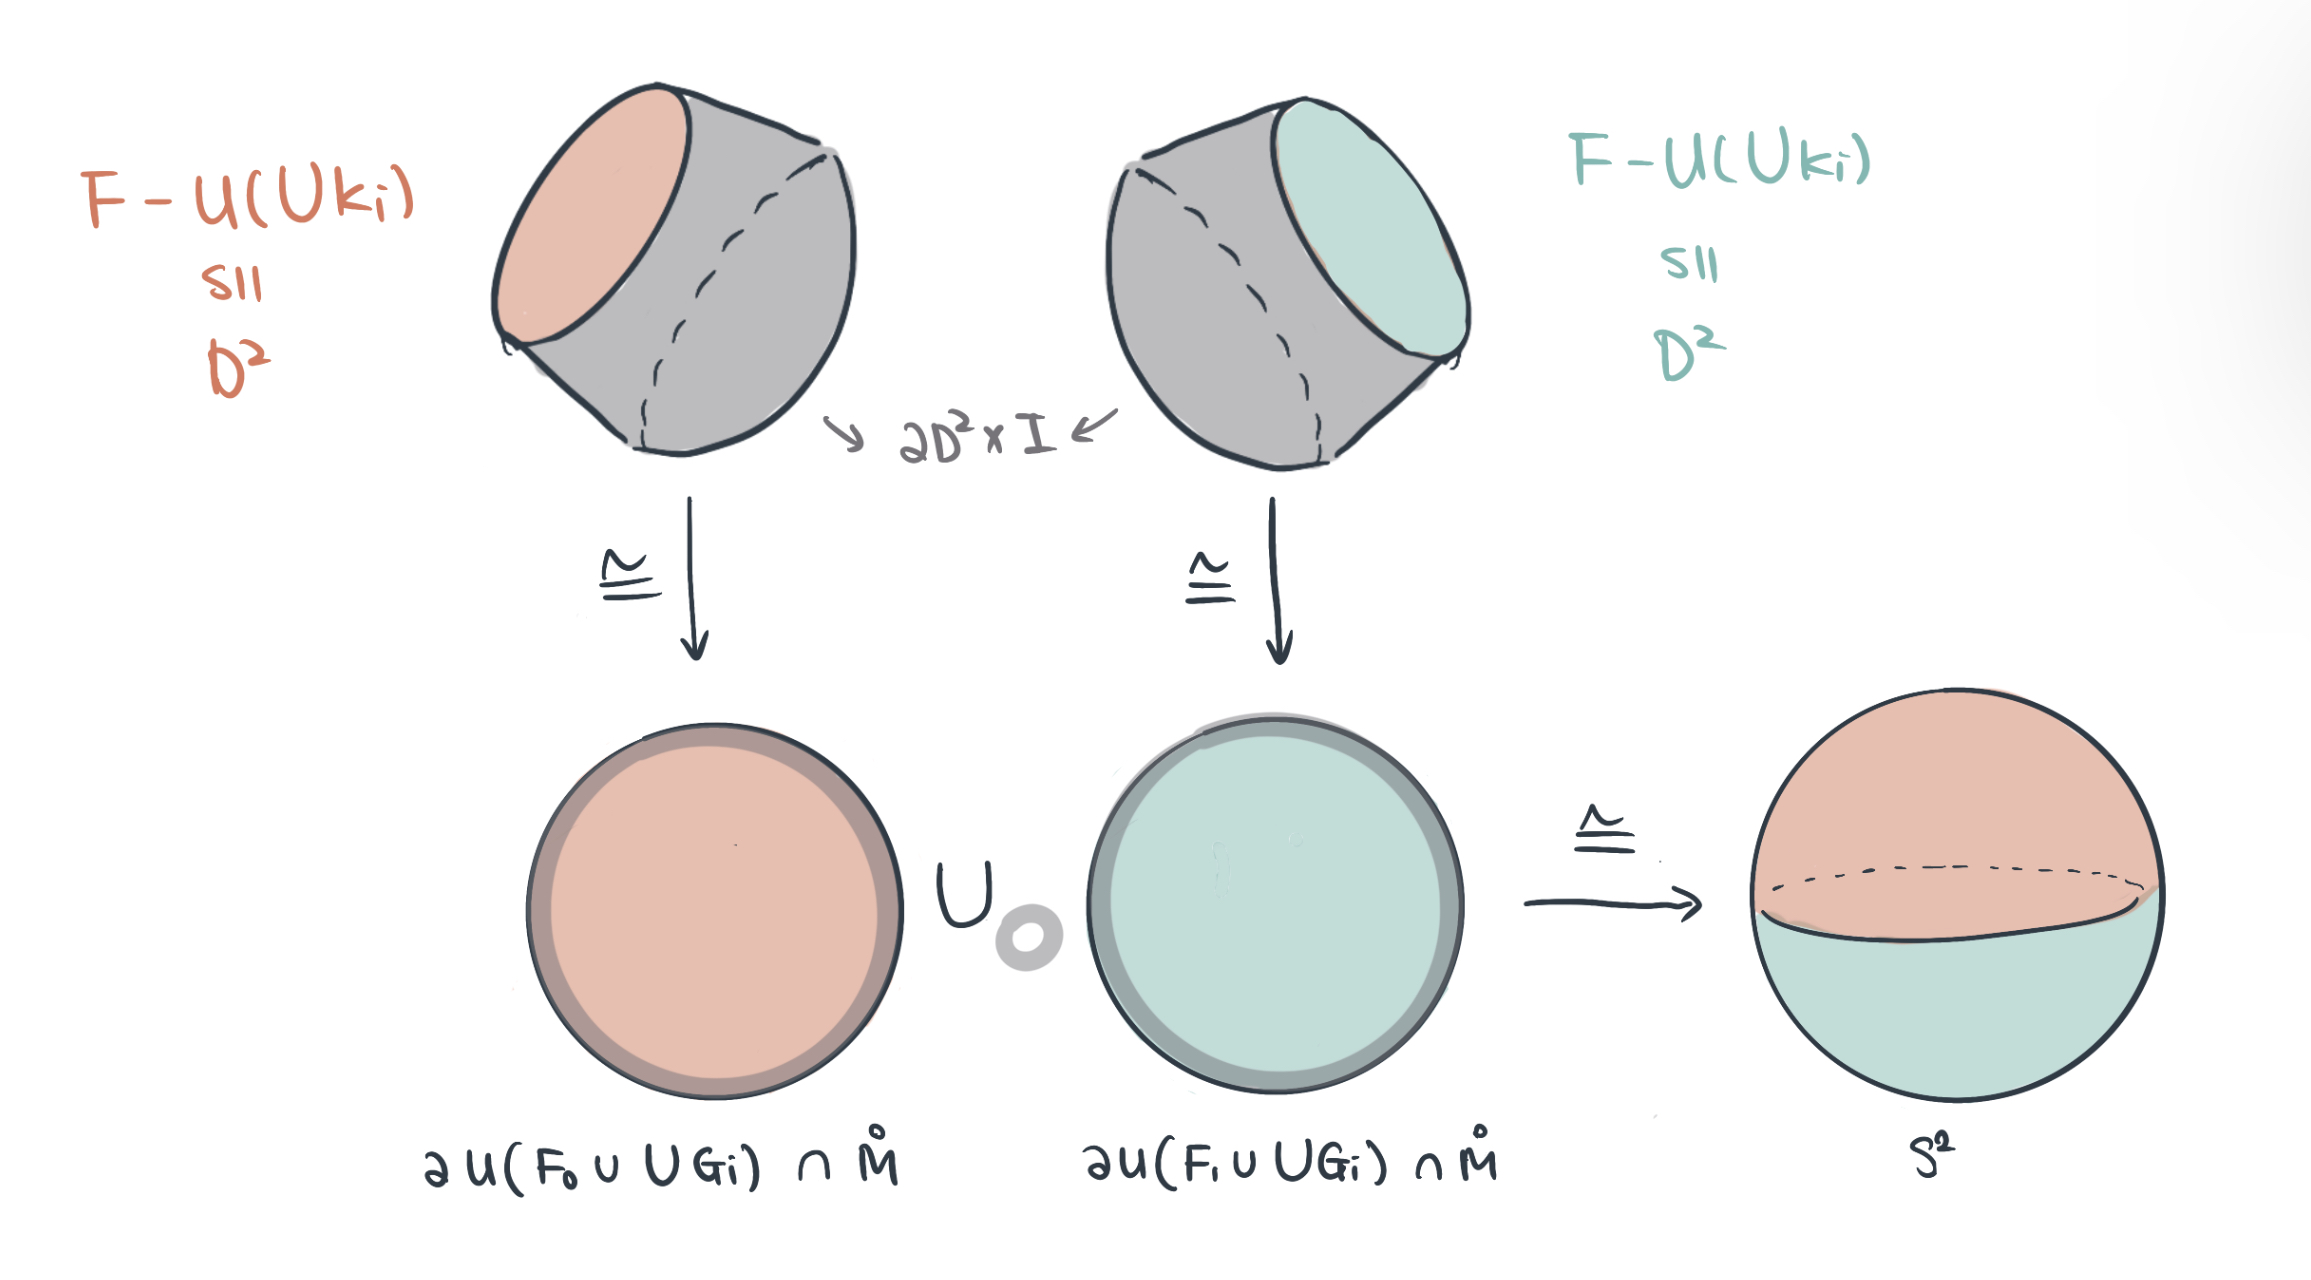
\includegraphics[width = 1\textwidth]{IMG2.png}
	 	\caption{bottle caps.}
	 	\label{fig:bottlecap}
	 \end{figure}

	 We have the regular neighborhood of a bunch of things and a ball, now what? I don't know. Time to sweep those under a rug and pretend this did not happen.
\end{proof}

After a lot of practices, we are now experts in cutting 3-manifold. It is time for the actual proof. 

\begin{proof}[Actual proof]
	Our strategy is trying to repeat the proof in the warm-up. When things don't work, we will change something and try to make them work. This sounds like a perfect plan and surely everything will work out nicely at the end. 

	Just like the good old time, suppose \(F\) is a genus \(g\) surface, we put a system of \(2g\) essential simple closed curves \(\{k_1, \ldots , k_{2g}\}\) on \(F\) such that \(k_i\) and \(k_j\) intersect once traversely if \(i = j \pm 1\), and they are disjoint otherwise. By assumption, for any essential simple closed curve \(k\) in \(F\), a non-null multiple \(k^n\) is homotopic to an essential curve \(k'\) in \(F'\). Here is the first difference: the mapping cylinder \(G\) for \(k^n\) and \(k'\) is not an embedding anymore, since \(k^n\) is not simple. We need the following theorem to resolve this issue. 

	\begin{sat}
		Let \(M\) be a compact, orientable 3-manifold. Let \(A\) be an annulus and \(c_1, c_2\) be its two boundary components. Let \(f: (A, \partial A) \to (M, \partial M)\) be an essential map such that \(f(c_1)\) does not meet \(f(c_2)\). Then there exists an essential embedding \(g: (A, \partial A) \to (M, \partial M)\) such that \(g(c_i)\) lies in any prespecified neighborhood of \(f(c_i)\) for \(i = 1, 2\). 
	\end{sat}

	Here, essential means \(\pi_1\)-injective and any simple arc connecting both boundary components of \(A\) does not homotope to an arc in \(\partial M\). The inclusion \(\iota\) of the mapping cylinder from \(k^n\) to \(k'\) is indeed essential, and \(\iota(k^n) \cap \iota(k') = \O\). Therefore, there exist embedded annuli \(G_1, \ldots, G_{2g}\) such that for each \(G_i\), its boundary components are homotopic to \(k_i\) in \(F\) and some simple essential closed curve \(k_i'\) in \(F'\).

	Now we have \(2g\) annuli. The next obstacle is that they can intersect in crazy ways, unlike before. Luckily, ``crazy'' was an exaggeration: A pair of annuli \(G_i, G_j\) will only intersect in 4 ways, and we only need to take care of 3 of the 4. If they intersect in an curve, the curve is either essential in both annuli or not essential in both annuli, since if not, we can find a disc in \(M\) with boundary \(k_i\) or \(k_j\), contradicting that \(F\) is incompressible. If \(G_i, G_j\) intersect in an arc and \(i \neq j\pm 1\), the arc will have both endpoint in \(F'\). If \(i = j\pm1\), then there is one intersection arc that connects both boundary components, we call that arc the nice arc. Note that in the warm-up, \(G_i\)'s only intersect at the nice arcs. We want our current system of \(G_i\)'s also only intersect at the nice arcs. 

	\begin{figure}
		\centering
		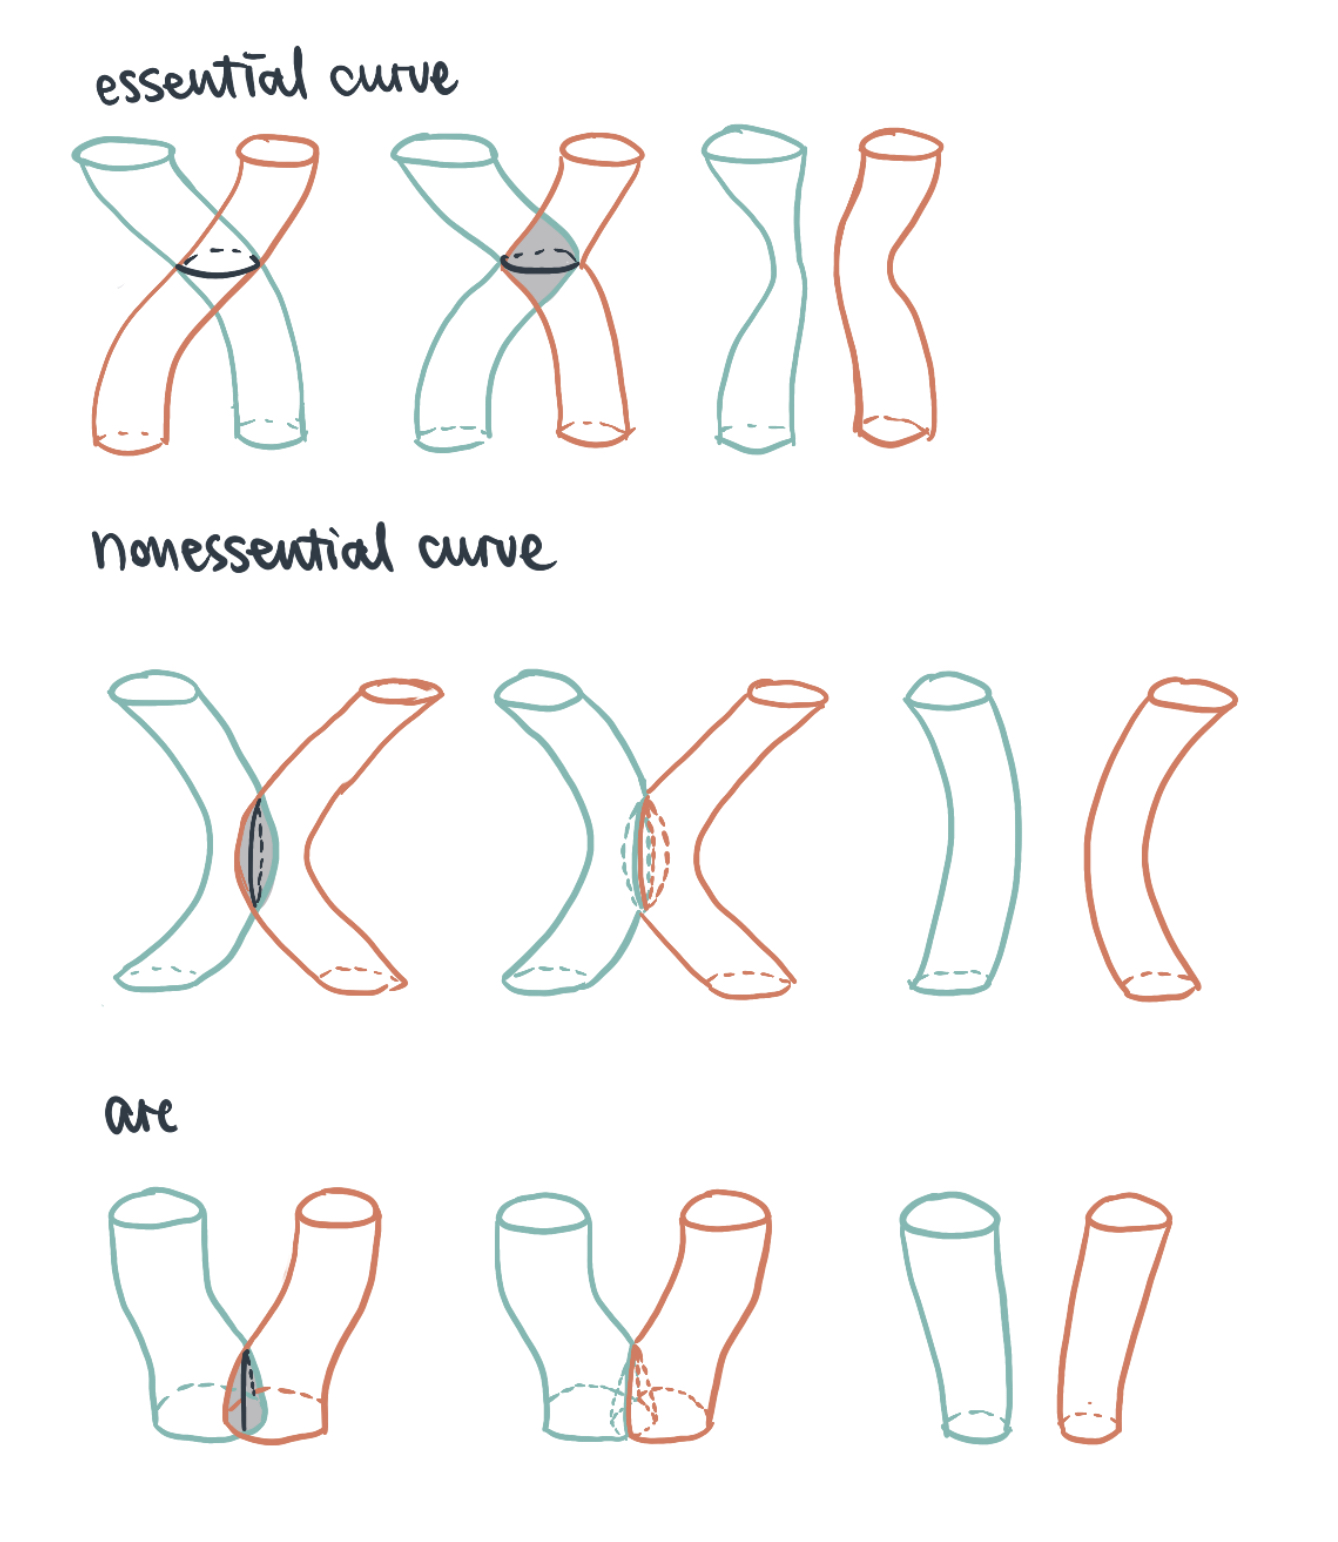
\includegraphics[width = 0.75\textwidth]{cut.jpeg}
		\caption{three types of surgeries}
		\label{fig:cuts}
	\end{figure}

	We will use the fact that \(M\) is irreducible and \(F'\) is incompressible to do surgeries on pairs of annuli. See Figure \ref{fig:cuts}. If \(G_i, G_j\) intersect at an essential curve in both annuli, we can cut along the curve and switch the bottom of two annuli. [I got confused here. Not sure why that resolves this intersection after switching.] If \(G_i, G_j\) intersect at a nonessential curve, the intersection bounds a disk on each annulus, so together these two discs glue to be a sphere which bounds a ball. This means there's no interesting topology there and we can safely wiggle the annuli to resolve this intersection. If \(G_i, G_j\) intersect at an arc, the arc cuts out a bigon from each annuli and they are glued to be an disc. Since \(F'\) is incompressible, \(\partial D\) is not an essential curve in \(F'\). Therefore we can also wiggle the annuli (not fixing boundary on \(F'\)) so that the intersection either disappears or turns into nonessential curve type.  Since there are only \(2g\) annuli and each pair intersects finite times (??), and each curve type surgery decreases the intersection numbers, we can eventually achieve our goal, that annuli only intersect at nice arcs.

	Everything looks so familiar and you might think we can do what we did in warm-up now. Not so fast. In warm-up, we know what \(F'\) is but now we don't, so we cannot safely conclude that  \(\partial U(F' \cup \bigcup G_i) \cap \mathring{M}\) (bottom bottle cap) is also homeomorphic to a disc. 
	However, the top bottle cap \(\partial U(F \cup \bigcup G_i) \cap \mathring{M}\) is still a disk. Since \(F'\) is incompressible, the boundary of the disk is non-essential in \(F'\). Thus \(F'\backslash \bigcup k_j'\) is a disk. Consequently, \(F' \cong F\) since they have the same fundamental group. 
	Now we can repeat the process in warm-up and get a regular neighborhood and a ball. 

	We come to the final stage of this proof. Using cell-complex, we can show that \(F \cup F' \cup \bigcup G_i\) is homeomorphic to \(F_0 \cup F_1 \cup \bigcup G_i\) in warm-up, since everything intersect in a very restricted way in both scenarios. [There are probably more concrete ways to show this.] Consequently, the regular neighborhood of these two are homeomorphic, and stay homeomorphic after gluing back the balls. Therefore \(M \cong F \times I\). 
\end{proof}


-----


Next step: Using this lemma to say something about hyperbolic 3-manifold \(M\) which has surface fundamental group.



\end{document}